\documentclass[conference]{IEEEtran}
\IEEEoverridecommandlockouts

\usepackage{cite}
\usepackage{amsmath,amssymb,amsfonts}
\usepackage{graphicx}
\usepackage{booktabs}
\usepackage{multirow}
\usepackage{xcolor}
\usepackage{tikz}
\usetikzlibrary{arrows.meta,positioning,fit,backgrounds,calc}
\usepackage[caption=false,font=footnotesize]{subfig}
\usepackage{url}

\newcommand{\xx}{\mathbf{x}}
\newcommand{\yy}{\mathbf{y}}
\newcommand{\zz}{\mathbf{z}}
\newcommand{\best}[1]{\textbf{#1}}

\begin{document}

\title{Safe Adaptive Quantization for Ultra-Low-Bitrate\\ Generative Image Compression}

\author{\IEEEauthorblockN{Anonymous Authors}
\IEEEauthorblockA{Paper ID: XXXX\\
Affiliation withheld for double-blind review}}

\maketitle

\begin{abstract}
Modern image compression methods are built from neural networks: instead of
hand-designed transforms, they learn to turn an image into a compact set of
features and to model the statistics of those features so they can be stored in
few bits. At very low bitrates, optimizing for pixel accuracy makes
reconstructions look blurry and unnatural, so recent methods attach a generative
decoder that \emph{synthesizes} realistic detail. This creates an opportunity: if
the decoder can plausibly invent texture on its own, the encoder need not spend
bits describing detail the decoder could reproduce anyway. We turn this into a
method. On top of an existing, \emph{frozen} generative compression model, we add
a small module that decides, for each region of the image, whether its fine detail
can be dropped without visibly hurting quality, and quantizes that region more
coarsely when it can. The decision is reconstructed by the decoder from
information it already receives, so nothing extra is transmitted, and the module
reduces to the original model when switched off. Trained with a criterion that
permits coarsening only where it saves bits without harming appearance, our
method---Safe Adaptive Quantization (SAQ)---reduces the rate at equal perceptual
quality by about $10\%$ in DISTS and $6\%$ in FID on the CLIC2020 and DIV2K
benchmarks, without retraining the underlying model. An analysis confirms that the
learned module preserves edges and texture while economizing on flat, predictable
regions.
\end{abstract}

\begin{IEEEkeywords}
Learned image compression, generative compression, perceptual quality, adaptive
quantization, ultra-low bitrate.
\end{IEEEkeywords}

\section{Introduction}
\label{sec:intro}
Image compression decides which information in a picture to keep and which to
discard. Modern systems learn this decision from data: a neural network maps an
image to a compact set of features, a second network models the probabilities of
those features so they can be written with few bits, and a decoder network
reconstructs the image. This paradigm, learned image compression (LIC), has grown
from transform autoencoders with hyperpriors~\cite{balle2017end,balle2018variational}
into strong systems whose entropy models exploit autoregressive, channel-wise, and
transformer-based context~\cite{minnen2018joint,minnen2020channel,cheng2020learned,he2022elic,liu2023tcm}.
These systems are tuned for rate--distortion, but at very low bitrates a
distortion objective rewards blurry, averaged reconstructions that look unnatural
to a human observer. This mismatch is formalized by the
rate--distortion--perception trade-off~\cite{blau2018perception,blau2019rethinking}
and has driven a shift toward \emph{generative} compression, where the decoder is
trained to produce realistic detail at a small rate cost~\cite{agustsson2019extreme,mentzer2020hific,muckley2023improving}.

A generative decoder changes what the bitstream must carry. Because the decoder
can synthesize plausible high-frequency content from a compact code, it no longer
needs every detail to be transmitted explicitly. Vector-quantized and diffusion
decoders push this idea to extreme rates: Generative Latent Coding
(GLC)~\cite{jia2024generative,qi2025generative} performs transform coding in the
latent space of a generative VQ autoencoder~\cite{esser2021taming} and reports
high realism below $0.05$~bpp, and diffusion codecs reconstruct recognizable
images at a few thousandths of a bit per pixel~\cite{yang2023lossy,careil2024towards}.

This raises a simple question that, to our knowledge, is rarely asked directly:
\emph{if the decoder can regenerate part of the detail, why spend the same
coding precision everywhere?} Spatially adaptive bit allocation is a classic
idea, but in LIC it is usually realized either by transmitting a content
importance map~\cite{li2018contentweighted}---which adds to the rate---or by
retraining the codec for each operating point~\cite{choi2019variable}. Neither
fits a setting where we want to exploit the recovery ability of an
\emph{existing, frozen} generative codec without paying for extra side
information.

We address exactly this setting. Our method, Safe Adaptive Quantization (SAQ),
learns \emph{where} the latent can be quantized more coarsely without perceptual
damage, and---crucially---makes that decision recomputable at the decoder so it
costs no bits. SAQ is a small module attached to a frozen GLC codec. From the
information the decoder already has (the transmitted hyper code and the partially
decoded latent), it predicts a per-region gate $\gamma\!\ge\!1$ that enlarges the
quantization step. Because $\gamma\!\ge\!1$, SAQ never codes the latent more
finely than the base codec, and a zero initialization makes it identical to GLC,
so any gain comes purely from coarsening where it is safe. To decide what is
safe, SAQ is trained with a benefit--cost teacher that rewards a larger gate only
where coarsening saves rate while keeping the reconstruction close to the
original.

Our contributions are:
\begin{itemize}
\item We show that a frozen state-of-the-art generative codec spends latent
precision on detail its own decoder can regenerate, and that this precision can
be reduced \emph{spatially} and \emph{without side information}.
\item We propose SAQ, a lightweight decoder-recomputable quantization gate
trained with a benefit--cost (safe-coarsening) teacher; it adds no side channel,
is monotone ($\gamma\!\ge\!1$), and reproduces the base codec at initialization.
\item Without retraining the base codec, SAQ reduces the Bj{\o}ntegaard
rate~\cite{bjontegaard2001calculation} by about $10\%$ (DISTS) and $6\%$ (FID) on
CLIC2020 and DIV2K, and we analyze where and why the savings arise.
\end{itemize}

\section{Related Work}
\label{sec:related}
\textbf{Learned image compression.}
End-to-end transform coding with hyperpriors~\cite{balle2017end,balle2018variational}
and increasingly expressive entropy
models~\cite{minnen2018joint,minnen2020channel,cheng2020learned,he2022elic,liu2023tcm}
defines the rate--distortion state of the art; we build on the open
CompressAI-style tooling~\cite{begaint2020compressai}. These works improve
$p(\yy)$ or the transform; we instead change \emph{how coarsely} parts of $\yy$
are quantized for a fixed codec.

\textbf{Perceptual and generative compression.}
Optimizing for realism rather than distortion improves low-rate visual
quality~\cite{blau2019rethinking}. GAN-based
codecs~\cite{agustsson2019extreme,mentzer2020hific,muckley2023improving} and
VQ-/diffusion-based generative
codecs~\cite{jia2024generative,qi2025generative,yang2023lossy,careil2024towards}
reach ultra-low bitrates by synthesizing detail. GLC~\cite{jia2024generative} is
our frozen base codec. SAQ is orthogonal: it is a bit-allocation layer that can
sit on such a codec to spend fewer bits where the generator already suffices.

\textbf{Adaptive bit allocation.}
Content-weighted coding transmits an importance map to allocate
bits~\cite{li2018contentweighted}, and conditional autoencoders enable
variable-rate coding~\cite{choi2019variable}. Unlike these, SAQ sends no map and
does not retrain the codec; its allocation is recomputed at the decoder, and it is
supervised to coarsen only where it is perceptually safe.

\begin{figure}[t]
\centering
\resizebox{\columnwidth}{!}{%
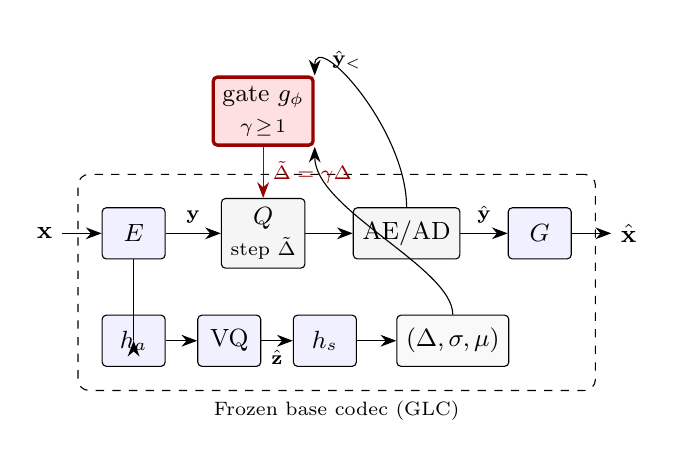
\begin{tikzpicture}[
  font=\small,
  block/.style={draw, rounded corners=1.5pt, minimum height=6.5mm, minimum width=8mm, align=center, fill=gray!8},
  frozen/.style={block, fill=blue!6},
  ours/.style={draw, rounded corners=1.5pt, minimum height=6.5mm, align=center, fill=red!12, very thick, draw=red!60!black},
  io/.style={align=center},
  >={Stealth[length=2mm]}]

  \node[io] (x) {$\xx$};
  \node[frozen, right=5mm of x] (enc) {$E$};
  \node[block, right=7mm of enc] (q) {$Q$\\\scriptsize step $\tilde\Delta$};
  \node[block, right=6mm of q] (ec) {AE/AD};
  \node[frozen, right=6mm of ec] (g) {$G$};
  \node[io, right=5mm of g] (xh) {$\hat\xx$};

  \draw[->] (x) -- (enc);
  \draw[->] (enc) -- node[above,font=\scriptsize]{$\yy$} (q);
  \draw[->] (q) -- (ec);
  \draw[->] (ec) -- node[above,font=\scriptsize]{$\hat\yy$} (g);
  \draw[->] (g) -- (xh);

  % hyper branch
  \node[frozen, below=7mm of enc] (he) {$h_a$};
  \node[frozen, right=4mm of he] (vq) {VQ};
  \node[frozen, right=4mm of vq] (hd) {$h_s$};
  \node[block, right=5mm of hd, fill=gray!5] (par) {$(\Delta,\sigma,\mu)$};
  \draw[->] (enc.south) |- (he);
  \draw[->] (he) -- (vq);
  \draw[->] (vq) -- node[below,font=\scriptsize]{$\hat\zz$} (hd);
  \draw[->] (hd) -- (par);

  % gate
  \node[ours, above=6.5mm of q] (gate) {gate $g_\phi$\\\scriptsize $\gamma\!\ge\!1$};
  \draw[->] (par.north) .. controls +(0,0.6) and +(0,-0.8) .. (gate.south east);
  \draw[->, red!60!black] (gate.south) -- node[right,font=\scriptsize]{$\tilde\Delta=\gamma\Delta$} (q.north);
  \draw[->] (ec.north) .. controls +(0,1.0) and +(0,0.6) .. node[above,font=\scriptsize,pos=0.6]{$\hat\yy_{<}$} (gate.north east);

  \begin{scope}[on background layer]
    \node[draw, dashed, rounded corners, fit=(enc)(q)(ec)(g)(he)(vq)(hd)(par), inner sep=3mm, label={[font=\scriptsize]below:Frozen base codec (GLC)}] {};
  \end{scope}
\end{tikzpicture}}
\caption{SAQ on a frozen generative codec. The hyper branch produces a
content-adaptive quantization step $\Delta$ (with scale $\sigma$ and mean $\mu$).
A small gate $g_\phi$ predicts $\gamma\!\ge\!1$ from information already available
at the decoder---the transmitted hyper code and the partially decoded latent
$\hat\yy_{<}$---and enlarges the step to $\tilde\Delta=\gamma\Delta$. The gate is
recomputed at the decoder, so no map is transmitted; $\gamma\!\equiv\!1$ recovers
the base codec.}
\label{fig:method}
\end{figure}

\section{Method}
\label{sec:method}

\subsection{Background: latent coding in a generative codec}
We build on GLC~\cite{jia2024generative}. An encoder maps the image $\xx$ to a
latent $\yy=E(\xx)$ in the space of a generative VQ
autoencoder~\cite{esser2021taming}; a generator reconstructs $\hat\xx=G(\hat\yy)$.
A hyper-analysis transform produces a summary $\zz$ that is vector-quantized and
transmitted as codebook indices; a hyper-synthesis transform turns the dequantized
$\hat\zz$ into a content-adaptive quantization step $\Delta$, a scale $\sigma$ and
a mean $\mu$ for the latent. Each latent element is coded as
\begin{equation}
r=\Big\lfloor \tfrac{y}{\Delta}-\mu \Big\rceil,\qquad
\hat y=\Delta\,(r+\mu),
\label{eq:base}
\end{equation}
where the residual $r$ is entropy-coded under a Gaussian model with scale
$\sigma$, and $\lfloor\cdot\rceil$ is rounding. The latent is decoded in four
spatial passes, so $\sigma$ and $\mu$ for later positions are conditioned on the
already-decoded latent. The side information ($\hat\zz$ indices) is small and, as
we confirm below, unchanged by our method.

\subsection{Safe adaptive quantization}
The step $\Delta$ in \eqref{eq:base} is already content-adaptive, but it is
optimized for the codec's own rate--distortion; it does not account for the fact
that the generator $G$ can regenerate some detail. SAQ inserts a multiplicative
gate. Let $c$ denote the information available at the decoder when a latent
position is coded: the hyper-derived parameters $(\Delta,\sigma,\mu)$ and the
partially decoded latent $\hat\yy_{<}$. A small network $g_\phi$ predicts
\begin{equation}
\gamma = 1+(\gamma_{\max}-1)\,\psi\!\big(g_\phi(c)\big)\in[1,\gamma_{\max}],
\label{eq:gate}
\end{equation}
where $\psi(\cdot)\in[0,1)$ is a smooth squashing function and $\gamma_{\max}$
caps the coarsening. The quantization step is replaced by $\tilde\Delta=\gamma\Delta$
in \eqref{eq:base}. Three properties make this usable on a frozen codec without
side information (Fig.~\ref{fig:method}):

\noindent\emph{(i) No side channel.} $c$ contains only signals the decoder also
has, so $\gamma$ is recomputed identically at decode time; nothing extra is
transmitted.

\noindent\emph{(ii) Monotonicity.} Since $\gamma\!\ge\!1$, the step never shrinks:
SAQ can only drop precision relative to GLC, never request more.

\noindent\emph{(iii) Exact fallback.} The final layer of $g_\phi$ is
zero-initialized, so $\gamma\!\equiv\!1$ at the start and SAQ reproduces GLC
exactly; any improvement is attributable solely to learned coarsening.

A complementary head, sharing the same decoder-available context $c$ and the same
zero-initialization, refines the entropy parameters $(\sigma,\mu)$ used to code
the residual. It carries no side information and tightens the entropy model; the
gate is the component that reallocates rate.

\subsection{Safe-coarsening objective}
A plain rate term would push $\gamma$ up everywhere and blur the image. The key is
to coarsen \emph{only where it is safe}. During training we therefore form a
benefit--cost target from the frozen base reconstruction. For a candidate
coarsening we measure, per region, the increase in fidelity error
($\Delta L_1$, $\Delta\mathrm{LPIPS}$ relative to GLC) and the rate it saves
($\Delta R$), and define a safety map
\begin{equation}
s=\sigma\!\Big(\tfrac{1}{\tau}\big[w_R\,\widetilde{\Delta R}-w_1\,\widetilde{\Delta L_1}-w_p\,\widetilde{\Delta\mathrm{LPIPS}}\big]\Big),
\label{eq:safe}
\end{equation}
where $\widetilde{(\cdot)}$ denotes per-image standardization and $\sigma$ is the
logistic function. A region is ``safe'' ($s\!\to\!1$) when coarsening saves bits
with little perceptual or fidelity damage. The full objective is
\begin{equation}
\mathcal{L}=R+\lambda_p\,\mathrm{LPIPS}(\xx,\hat\xx)+\lambda_s\,\mathrm{BCE}\!\big(\psi(g_\phi(c)),s\big)+\lambda_\gamma(\bar\gamma-\tau_\gamma)^2,
\label{eq:loss}
\end{equation}
where $R$ is the estimated rate, the third term aligns the gate with the safety
map, and the last term sets the operating point through a target mean gate
$\tau_\gamma$ (a single scalar that trades rate against quality). The base codec
stays frozen, and a learned rate embedding lets one SAQ module serve the four
operating points of GLC. We use LPIPS~\cite{zhang2018unreasonable} as the
perceptual term; DISTS and FID are reserved for evaluation.

\section{Experiments}
\label{sec:exp}

\subsection{Setup}
\textbf{Base codec and training.} We attach SAQ to the official GLC image
codec~\cite{jia2024generative} and keep it frozen; only the SAQ heads (about
$6\%$ of the backbone parameters) are trained, on
OpenImages~\cite{kuznetsova2020open}. We report the four GLC operating points.

\textbf{Datasets.} Our rate--perception evaluation uses the CLIC2020 test set
(428 professional and mobile images)~\cite{clic2020} and the DIV2K validation set
(100 images)~\cite{agustsson2017ntire}; we use Kodak (24
images)~\cite{kodak1993} for the gate analysis and qualitative examples. All
images are coded at full resolution.

\textbf{Metrics.} Following the perceptual-compression literature, our primary
metrics are DISTS~\cite{ding2022image} and FID~\cite{heusel2017gans}, which
correlate with low-rate visual quality; we also report
LPIPS~\cite{zhang2018unreasonable} and KID~\cite{binkowski2018demystifying}, and
PSNR/MS-SSIM as distortion diagnostics. FID/KID use $256\!\times\!256$ patches.
We summarize rate--quality with Bj{\o}ntegaard delta
rate~\cite{bjontegaard2001calculation} (BD-rate), where a negative value means
fewer bits at equal quality.

\subsection{Rate--perception performance}
Table~\ref{tab:bdrate} reports BD-rate against the frozen GLC codec, and
Fig.~\ref{fig:rd} shows the corresponding curves. SAQ moves the
rate--perception curve left on both datasets: it needs $9.8\%$ and $10.4\%$ fewer
bits at equal DISTS, and $6.4\%$ and $5.6\%$ fewer bits at equal FID, on CLIC2020
and DIV2K. KID improves consistently ($-4.7\%$/$-5.0\%$). LPIPS is essentially
unchanged (Fig.~\ref{fig:rd}, right), which we attribute to its sensitivity to
the slight smoothing introduced by coarsening; we therefore do not claim a gain on
every metric and keep LPIPS as a neutral diagnostic. Because the gate sends no
side information and leaves the hyper code untouched, the side-information rate is
identical to GLC ($0.0035$~bpp on both sets); all savings come from the latent.
Fig.~\ref{fig:qual} shows the effect visually: at the top operating point SAQ
matches GLC at the same DISTS while using $8$--$9\%$ fewer bits.

\begin{table}[t]
\centering
\caption{BD-rate (\%) vs.\ the frozen GLC codec~\cite{jia2024generative}.
Negative is better (fewer bits at equal quality). DISTS and FID are the primary
perceptual metrics. ``w/o safe teacher'' trains the same gate without the
benefit--cost target of \eqref{eq:safe}.}
\label{tab:bdrate}
\setlength{\tabcolsep}{4.5pt}
\renewcommand{\arraystretch}{1.15}
\begin{tabular}{llrrrr}
\toprule
Dataset & Method & DISTS & LPIPS & FID & KID \\
\midrule
\multirow{2}{*}{CLIC2020}
 & SAQ, w/o safe teacher & $-8.37$ & $+0.68$ & $-5.50$ & $-4.39$ \\
 & \best{SAQ (full)}     & \best{$-9.76$} & $+0.05$ & \best{$-6.42$} & \best{$-4.65$} \\
\midrule
\multirow{2}{*}{DIV2K}
 & SAQ, w/o safe teacher & $-9.20$ & $-0.05$ & $-5.13$ & $-1.23$ \\
 & \best{SAQ (full)}     & \best{$-10.37$} & \best{$-0.49$} & \best{$-5.64$} & \best{$-4.98$} \\
\bottomrule
\end{tabular}
\end{table}

\begin{figure*}[t]
\centering
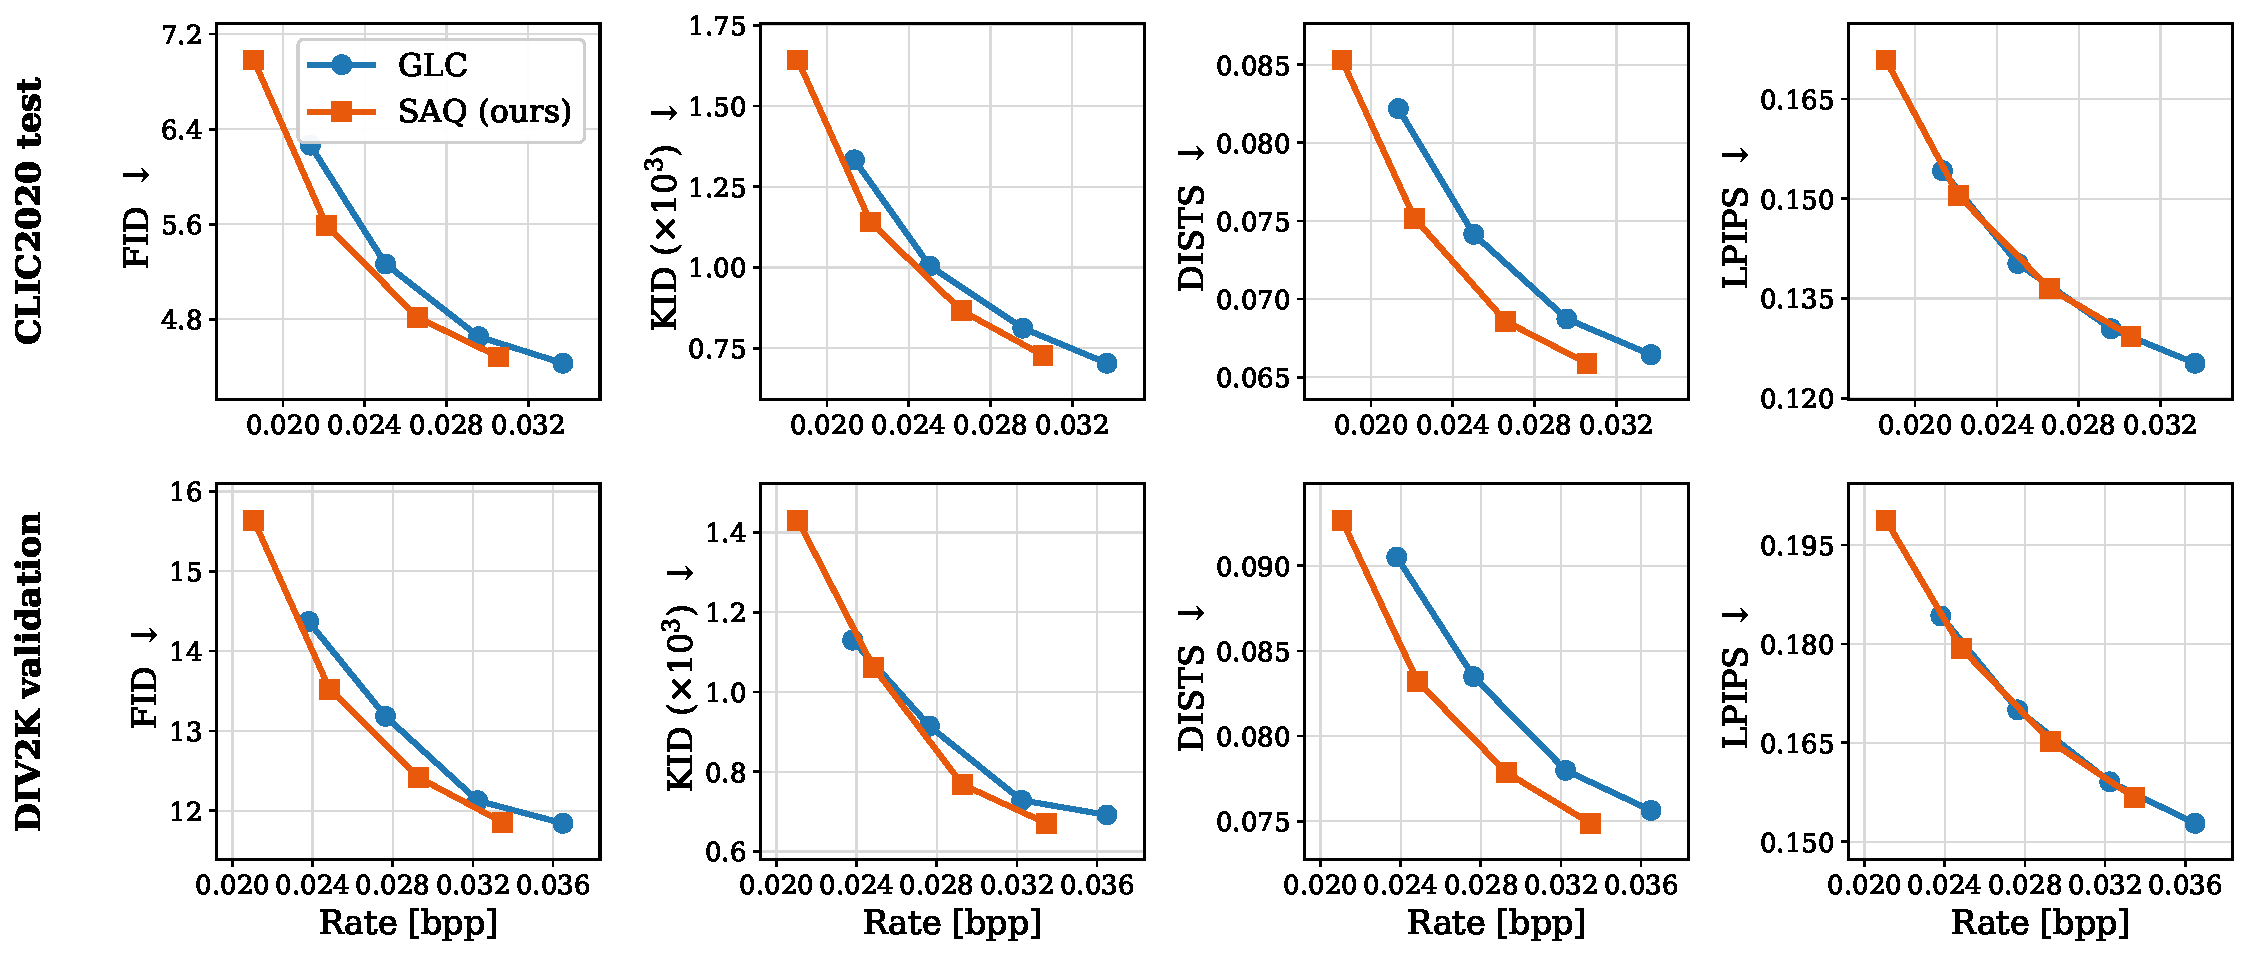
\includegraphics[width=\textwidth]{figures/rd_curves.pdf}
\caption{Rate--quality curves over the four operating points, for two
distribution metrics (FID, KID) and two full-reference perceptual metrics (DISTS,
LPIPS); lower-left is better. At a fixed quality, SAQ (orange) lies to the left of
GLC (blue), i.e.\ it needs fewer bits for the same FID, KID and DISTS on both
datasets. LPIPS, which is sensitive to mild smoothing, stays on the GLC curve.
KID is scaled by $10^3$.}
\label{fig:rd}
\end{figure*}

\begin{figure}[t]
\centering
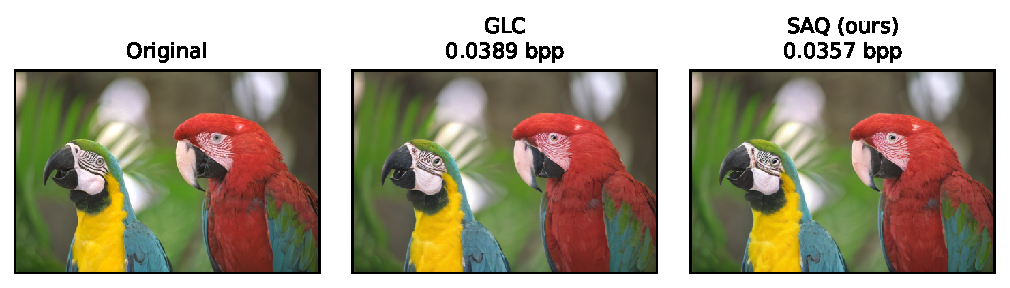
\includegraphics[width=\columnwidth]{figures/qualitative.pdf}
\caption{Reconstruction at the top operating point (Kodak, \texttt{kodim23}).
SAQ matches the frozen GLC codec in DISTS ($0.068$ for both) while spending
$8.3\%$ fewer bits; the side information is unchanged. Best viewed zoomed in.}
\label{fig:qual}
\end{figure}

\subsection{Effect of the safe-coarsening teacher}
The lower rows of Table~\ref{tab:bdrate} ablate the benefit--cost target of
\eqref{eq:safe}. Training the same gate without it---i.e.\ letting the rate term
distribute coarsening on its own---already helps, but the safety teacher improves
the DISTS BD-rate from $-8.4\%$ to $-9.8\%$ on CLIC2020 and from $-9.2\%$ to
$-10.4\%$ on DIV2K, with matching FID and KID gains. Telling the gate \emph{where}
coarsening is safe, rather than only \emph{how much} to coarsen on average, is
what turns a generic rate knob into a useful spatial allocation.

\subsection{What does the gate learn?}
Fig.~\ref{fig:gate} visualizes $\gamma$ at the highest rate. Coarsening
concentrates on flat, predictable regions (walls, sky, road) and backs off on
edges, text, and fine texture. We quantify this on Kodak by correlating $\gamma$
with local statistics of the image and of the base reconstruction. Averaged over
the $24$ images, the gate is negatively correlated with the base reconstruction
error ($-0.51$), local texture variance ($-0.47$), and gradient magnitude
($-0.52$): it raises precision-saving exactly where GLC is already accurate and
the content is smooth. Regions in the top gate quartile have less than half the
reconstruction error of the bottom quartile ($0.030$ vs.\ $0.074$). This is the
intended mechanism: spend bits on residual the generator cannot infer, and
coarsen the rest.

\begin{figure}[t]
\centering
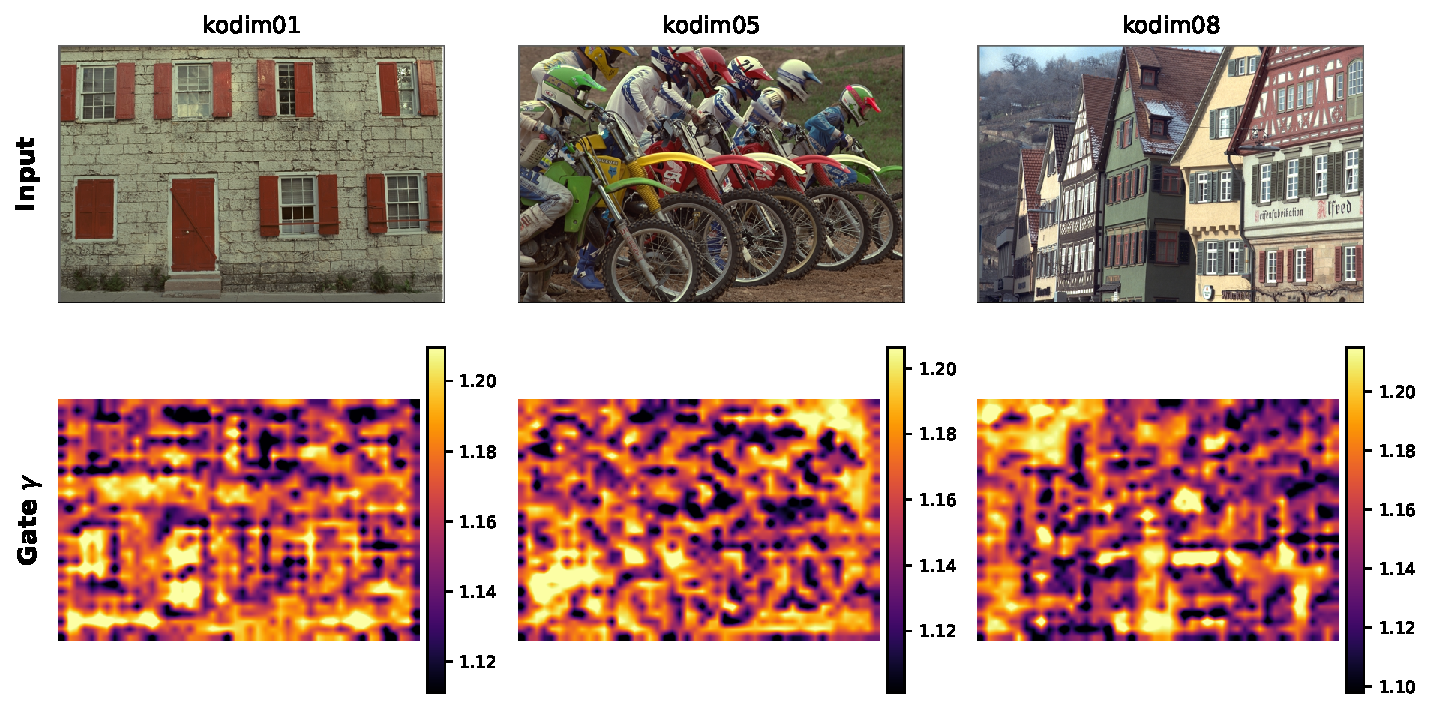
\includegraphics[width=\columnwidth]{figures/gate_map.pdf}
\caption{Learned gate $\gamma$ (higher\,$=$\,coarser) at the highest rate. The
gate enlarges the quantization step on flat regions (walls, road) and protects
edges, windows, and texture.}
\label{fig:gate}
\end{figure}

\subsection{Complexity}
SAQ keeps the GLC backbone frozen and adds only lightweight heads
($\approx\!6\%$ of the backbone parameters; the gate alone is $<\!3\%$). The
gate is a small convolutional network evaluated alongside the existing entropy
model, so it adds negligible cost to encoding and decoding and requires no
change to the bitstream format.

\section{Conclusion}
\label{sec:conclusion}
We presented Safe Adaptive Quantization, a side-information-free way to reallocate
coding precision in a frozen generative image codec. SAQ learns a
decoder-recomputable gate that coarsens the latent only where coarsening is
perceptually safe, supervised by a benefit--cost teacher. It reduces the
Bj{\o}ntegaard rate by about $10\%$ in DISTS and $6\%$ in FID on CLIC2020 and
DIV2K, with no change to the base codec and no extra bits, and the learned gate
demonstrably targets predictable, low-error regions. The principle---reserve bits
for what the generator cannot regenerate---is general, and SAQ realizes it as a
drop-in layer.

\textbf{Scope and future work.} We study the ultra-low-bitrate regime of one base
codec; LPIPS is left essentially unchanged, reflecting the perception--distortion
nature of coarsening. Promising directions are learning to \emph{synthesize} the
omitted residual at the decoder rather than only dropping it, and applying the
same side-information-free gate to other generative and diffusion codecs.

\bibliographystyle{IEEEtran}
\bibliography{refs}

\end{document}
